\section{Theory \label{sec:VT-theory}}

Two orthogonal standing waves excited at the same frequency $f$ and with a 
relative phase shift $\zeta$ exert a torque on spherical particles. Under these 
conditions, an acoustic streaming field is formed inside the viscous boundary 
layer

\begin{equation}
    \delta = \sqrt{\frac{\mu_{f}}{\rho_{f}\,\pi\,f}}
    \label{eq:VT-delta}
\end{equation}

at the fluid-particle interface, where $f$ is the frequency (of excitation), 
$\mu_{f}$ the dynamic fluid viscosity, and $\rho_{f}$ the density of the fluid. 
The resulting viscous surface stress on the particle results in a non-zero 
torque. This torque is called the acoustic VT and is qualitatively shown in 
\cref{fig:Fig1} for two orthogonal standing waves with a phase shift of $\zeta = 
\sfrac{\pi}{2}$.

%%%%%%%%%%%
\begin{figure}
    \centering
    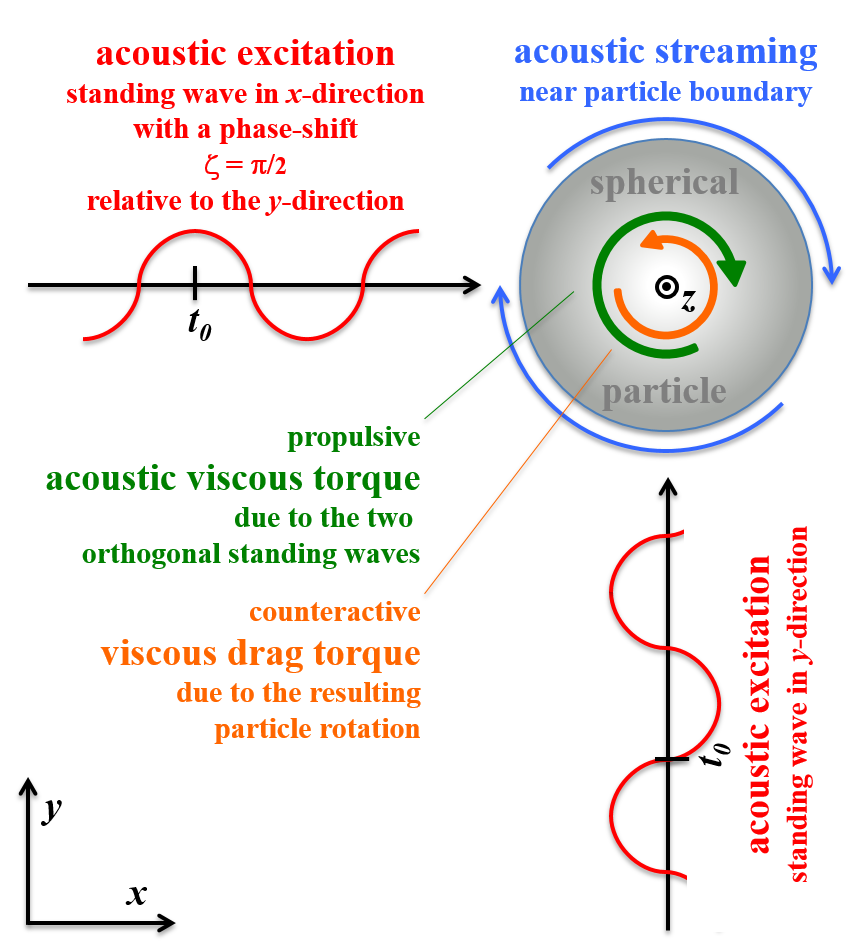
\includegraphics[width=84mm]{Fig1.png}
    \caption{Schematic of the time-averaged acoustic VT acting on a sphere. At a 
    constant rotational rate $\Omega$ of the particle the propulsive acoustic VT 
is in balance with its counteracting viscous drag torque.\label{fig:Fig1}}
\end{figure}%
%%%%%%%%%%%

The analytical solution for the total time-averaged VT 
$\Gamma_{\text{tot}}(\Omega)$ on a small rotating spherical particle 
($R\ll\lambda=\sfrac{c_f}{f}$) within two orthogonal plane standing waves is 

%%%%%%%%%%%%%%%%%%%
\begin{equation}
  \label{eq:VT-Eq1}
  \eqalign{
     \fl &\Gamma_{\text{tot}}(\Omega) = \\
     \fl &= \frac{3}{4} \frac{\delta S_s A_{X} A_{Y}}{\rho_{f} c_{f}^{2}} \sin\zeta \cos(kX)
     \cos(kY) - 8 \pi \mu_f R^3\,\Omega \\
     &= \Gamma_{\text{IN}} - \tilde{D}\,\Omega
  }
\end{equation}
%%%%%%%%%%%%%%%%%%%
where $S_s$ is the sphere surface area, and $c_f$ the speed of sound of the 
fluid, $k=\sfrac{2\pi}{\lambda}$ the wavenumber in the fluid, and ($A_{X}$; 
$A_{Y}$) the pressure amplitudes of the two orthogonal standing waves 
\cite{Wang, Lamprecht}.  The phase shift $\zeta$ and the sphere position 
($X$;$Y$) determine the rotation direction.  The result of 
$\Gamma_{\text{tot}}(\Omega)$ can be split up into a torque driven by the 
acoustic excitation $\Gamma_{\text{IN}} \propto R^{2}$ and a viscous drag torque 
$\tilde{D}\,\Omega \propto R^{3}$ related to Stokes drag \cite{Lamprecht}. In 
the theory of \citeauthor{Nyborg} \cite{Nyborg} and \citeauthor{Wang} 
\cite{Wang}, the particle rotation was not considered in their analysis of the 
acoustic VT $\Gamma_{\text{IN}}$.  However, \citeauthor{Lamprecht} 
\cite{Lamprecht} introduced a moving boundary of the particle so that the 
driving $\Gamma_{\text{IN}}$ appears independently of the rotational rate 
$\Omega$. The rotational axis of the particle is always perpendicular to both 
directions of the incident waves and its rotational rate is limited by Stokes 
drag coefficient $\tilde{D} = 8 \pi \mu_f R^3$. The steady-state rotational rate 
$\finalOmega$ is defined as
%%%%%%%%%%%%%%%%%%%
\begin{equation}
  \label{eq:VT-AcGovEqConti}
  \finalOmega=\frac{\Gamma_{\text{IN}}}{\tilde{D}}.
\end{equation}
%%%%%%%%%%%%%%%%%%%
Since $\finalOmega \propto \sfrac{1}{R}$ \cite{Lamprecht}, bigger particles will 
reach a lower steady-state rotational rate $\finalOmega$. This occurs for the 
equilibrium state $\Gamma_{\text{IN}}(t=t^\star)= \tilde{D} (t = t^\star )$.  
After $ t^\star = \SI{0.5}{\milli\second}$ a \SI{100}{\micro\meter} large 
particle rotates with the steady-state rate of $\SI{11.33}{\hertz}$
(\SI{680}{\rpm}) at an acoustic pressure amplitude of \SI{171}{\kilo\pascal} 
\cite{lamprecht2015}. Please note that the time constant $\tau \approx 
t^{\star}$ is proportional to $R^2$ \cite{lamprecht2015}, so a particle with 
$2\,R=\SI{2.06}{\um}$ reaches the equilibrium in less than 
\SI{1}{\micro\second}. \citeauthor{hahn2016} \cite{hahn2016} showed numerically 
that the analytical and the numerical results can differ by orders of magnitude 
for $\normBdLayer > 1$ and water as fluid. For acoustic particle manipulation in 
water, the differences between the analytical solution and the numerical results 
become negligible for particles with a normalized viscous boundary layer 
$\normBdLayer < \sfrac{1}{15}$. In addition, the analytical predictions neglect 
the density ratio $\tilde{\rho} = \sfrac{\rho_{\text{s}}}{\rho_{\text{f}}}$ 
between the particle and the surrounding fluid.  \citeauthor{hahn2016} 
\cite{hahn2016} concluded that the density ratio $\tilde{\rho}$ has a 
non-negligible effect on the magnitude of the acoustic VT and that depending on 
this ratio even the direction of the torque can change.
